\documentclass{ctexbook}
\usepackage{graphicx}
\usepackage{hyperref}
\usepackage{listings}
\usepackage{xcolor}
\usepackage{geometry}
\geometry{a4paper, margin=1in}

\title{MQTT}
\author{}
\date{}

\begin{document}
\maketitle
\tableofcontents

\chapter{MQTT: The Standard for IoT Messaging}
MQTT: The Standard for IoT Messaging 物联网消息传递的标准

MQTT is an OASIS standard messaging protocol for Internet of Things (IoT). It is designed as an extremely lightweight publish/subscribe messaging transport that is ideal for connecting remote devices with a small code footprint and minimal network bandwidth. MQTT today is used in a wide variety of industries, such as automotive, manufacturing, telecommunications, oil and gas, etc.

MQTT 是物联网（IoT）的 OASIS 标准消息传递协议。它被设计为一种非常轻量级的发布/订阅消息传输，非常适合以较小的代码占用和最小的网络带宽连接远程设备。MQTT 如今用于各种行业，如汽车、制造业、电信、石油和天然气等。

\section{Why MQTT?}
Why MQTT? 为什么选择 MQTT？

\subsection{Lightweight and Efficient}
Lightweight and Efficient 轻巧高效

MQTT clients are very small, require minimal resources so can be used on small microcontrollers. MQTT message headers are small to optimize network bandwidth.

MQTT 客户端非常小，需要最少的资源，因此可以在小型微控制器上使用。MQTT 消息头很小，以优化网络带宽。

\subsection{Bi-directional Communications}
Bi-directional Communications 双向通信

MQTT allows for messaging between device to cloud and cloud to device. This makes for easy broadcasting messages to groups of things.

MQTT 允许设备到云和云到设备之间的消息传递。这使得很容易将消息广播到一组事物。

\subsection{Scale to Millions of Things}
Scale to Millions of Things 扩展到数百万件事物

MQTT can scale to connect with millions of IoT devices.

MQTT 可以扩展到连接数百万个物联网设备。

\subsection{Reliable Message Delivery}
Reliable Message Delivery 可靠的消息传递

Reliability of message delivery is important for many IoT use cases. This is why MQTT has 3 defined quality of service levels: 0 - at most once, 1- at least once, 2 - exactly once

消息传递的可靠性对于许多物联网用例都很重要。这就是为什么 MQTT 有 3 个定义的服务质量级别：0 - 最多一次，1 - 至少一次，2 - 正好一次

\subsection{Support for Unreliable Networks}
Support for Unreliable Networks 支持不可靠的网络

Many IoT devices connect over unreliable cellular networks. MQTT's support for persistent sessions reduces the time to reconnect the client with the broker.

许多物联网设备通过不可靠的蜂窝网络连接。MQTT 对持久会话的支持减少了重新连接客户端和代理的时间。

\subsection{Security Enabled}
Security Enabled 启用安全的

MQTT makes it easy to encrypt messages using TLS and authenticate clients using modern authentication protocols, such as OAuth.

MQTT 可以轻松地使用 TLS 加密消息，并使用现代身份验证协议（如 OAuth）对客户端进行身份验证。

\section{MQTT Publish / Subscribe Architecture}
MQTT Publish / Subscribe Architecture MQTT 发布/订阅架构

\begin{figure}[htbp]
\centering
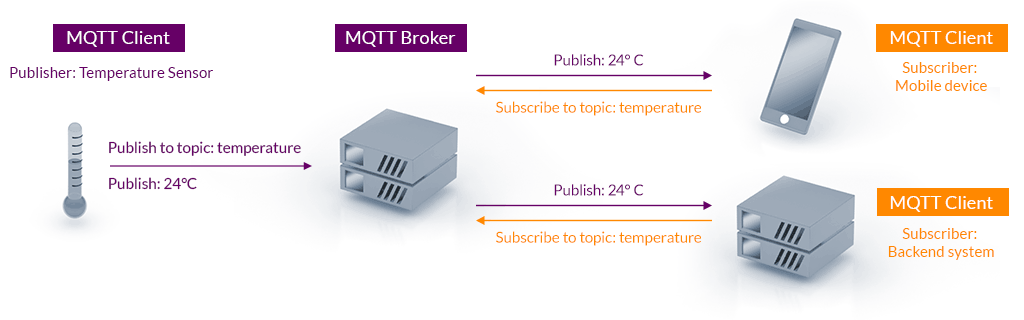
\includegraphics[width=0.8\textwidth]{Images/mqtt-publish-subscribe.png}
\caption{MQTT Publish / Subscribe Architecture}
\end{figure}

\section{MQTT in Action}
MQTT in Action MQTT 在行动

MQTT is used in a wide variety of industries:
MQTT 用于各种行业：

\begin{itemize}
\item Automotive 汽车
\item Logistics 物流
\item Manufacturing 制造
\item Smart Home 智能家居
\item Consumer Products 消费产品
\item Transportation 运输
\end{itemize}

\section{MQTT Specifications}
MQTT Specifications MQTT 规范

MQTT is an OASIS standard. The specification is managed by the OASIS MQTT Technical Committee.

MQTT 是 OASIS 标准。该规范由 OASIS MQTT 技术委员会管理。

\subsection{MQTT 5 Specification}
MQTT 5 Specification MQTT 5 规范

MQTT 5 Specification is an OASIS Standard. 

MQTT 5 规范是 OASIS 标准。

\subsection{MQTT 3.1.1 Specification}
MQTT 3.1.1 Specification MQTT 3.1.1 规范

MQTT 3.1.1 Specification is an older ISO and OASIS Standard. 

MQTT 3.1.1 规范是较旧的 ISO 和 OASIS 标准。

\subsection{MQTT 3.1 Specification}
MQTT 3.1 Specification MQTT 3.1 规范

\subsection{MQTT-SN v1.2}
MQTT-SN v1.2 MQTT-SN v1.2

MQTT for Sensor Networks is aimed at embedded devices on non-TCP/IP networks, such as Zigbee. MQTT-SN is a publish/subscribe messaging protocol for wireless sensor networks (WSN), with the aim of extending the MQTT protocol beyond the reach of TCP/IP infrastructure for Sensor and Actuator solutions. 

MQTT for Sensor Networks 针对非 TCP/IP 网络上的嵌入式设备，如 Zigbee。MQTT-SN 是用于无线传感器网络（WSN）的发布/订阅消息传递协议，旨在将 MQTT 协议扩展到 TCP/IP 基础设施之外，用于传感器和执行器解决方案。

\section{MQTT Software}
MQTT Software MQTT 软件

\subsection{Servers / Brokers}
Servers / Brokers 服务器/代理

\subsubsection{Ably MQTT Broker}
Ably MQTT Broker Ably MQTT 代理

Ably provides an MQTT broker and protocol adapter that is able to translate back and forth between MQTT and Ably's own protocol. It provides support for WebSockets, HTTP, SSE, STOMP, AMQP, and many more. Ably provides an interoperable, globally-distributed realtime messaging infrastructure layer.

Ably 提供了一个 MQTT 代理和协议适配器，能够在 MQTT 和 Ably 自己的协议之间来回转换。它支持 WebSockets、HTTP、SSE、STOMP、AMQP 等多种协议。Ably 提供了一个可互操作的、全球分布的实时消息传递基础设施层。

\subsubsection{Akiro MQTT Broker}
Akiro MQTT Broker Akiro MQTT 代理

Akiro MQTT Broker is a high scale MQTT broker with support for more than 20 Million active MQTT connections with over 1 Million messages per second. It's written in Java with Vert.X's async paradigm. Akiro clients can be used to communicate with the free to use Akiro SaaS MQTT Broker. Akiro supports MQTT, Websockets over MQTT, HTTP over MQTT, DLMS, OCPP with TLS support.

Akiro MQTT Broker 是一个高规模的 MQTT 代理，支持超过 2000 万个活跃的 MQTT 连接，每秒处理超过 100 万条消息。它是用 Java 编写的，使用 Vert.X 的异步范式。Akiro 客户端可用于与免费使用的 Akiro SaaS MQTT 代理进行通信。Akiro 支持 MQTT、MQTT 上的 Websockets、MQTT 上的 HTTP、DLMS、OCPP，并支持 TLS。

\subsubsection{Apache ActiveMQ}
Apache ActiveMQ Apache ActiveMQ

Details of "classic" ActiveMQ's support for MQTT are available here.

"经典" ActiveMQ 对 MQTT 支持的详细信息可在此处找到。

\subsubsection{Apache ActiveMQ Artemis}
Apache ActiveMQ Artemis Apache ActiveMQ Artemis

The "next generation" of ActiveMQ, Artemis is a multi protocol messaging broker that supports MQTT.

ActiveMQ 的"下一代"版本，Artemis 是一个支持 MQTT 的多协议消息代理。

\subsubsection{async\_mqtt}
async\_mqtt async\_mqtt

An open-source MQTT broker using C++17 that supports MQTT v3.1.1 and v5.0. It also supports TLS, WebSocket, and multi-core scale-out. Licensed under the Boost Software License - Version 1.0.

一个使用 C++17 的开源 MQTT 代理，支持 MQTT v3.1.1 和 v5.0。它还支持 TLS、WebSocket 和多核扩展。根据 Boost 软件许可证 - 版本 1.0 授权。

\subsubsection{Bevywise CrystalMQ}
Bevywise CrystalMQ (Formerly MQTTRoute) Bevywise CrystalMQ（原名 MQTTRoute）

CrystalMQ, A high-performance MQTT broker designed for large-scale IoT deployments. Supports millions of connections with advanced features like multi-tenancy, clustering for high availability, and robust security controls. Ideal for industries needing real-time, low-latency communication. Broker can be customized to write data to any data store using standard connectors or custom implementations. Try the fully FREE version here.

CrystalMQ，一个为大规模物联网部署设计的高性能 MQTT 代理。支持数百万个连接，具有多租户、高可用性集群和强大的安全控制等高级功能。非常适合需要实时、低延迟通信的行业。代理可以使用标准连接器或自定义实现进行定制，将数据写入任何数据存储。在此处尝试完全免费的版本。

\subsubsection{Apache BifroMQ}
Apache BifroMQ Apache BifroMQ

Apache BifroMQ is a distributed MQTT messaging middleware optimized for high-performance scenarios. Its key feature is native multi-tenancy, enabling efficient resource sharing and strict workload isolation across tenants. The architecture incorporates a purpose-built distributed storage engine, minimizing dependency on external middleware components, even under heavy load. BifroMQ is particularly well-suited for building large-scale IoT infrastructures and messaging platforms, offering scalable, cloud-native, and serverless deployment options for demanding production environments.

Apache BifroMQ 是一个针对高性能场景优化的分布式 MQTT 消息传递中间件。其关键特性是原生多租户，能够在租户之间实现高效的资源共享和严格的工作负载隔离。该架构包含一个专用的分布式存储引擎，即使在重负载下也能最大限度地减少对外部中间件组件的依赖。BifroMQ 特别适合构建大规模物联网基础设施和消息传递平台，为要求苛刻的生产环境提供可扩展的、云原生的和无服务器的部署选项。

\subsubsection{Cassandana}
Cassandana Cassandana

Cassandana is an open source MQTT message broker which is entirely written in Java. This project began its life as a fork of Moquette, and later underwent some cleanup, optimization and adding extra features. Now it's ready to work as an enterprise message broker.

Cassandana 是一个完全用 Java 编写的开源 MQTT 消息代理。该项目始于 Moquette 的一个分支，后来进行了一些清理、优化和添加额外功能。现在它已准备好作为企业消息代理工作。

\subsubsection{Coreflux}
Coreflux Coreflux

Coreflux is a Data Hub, based on MQTT 3.1.1 and 5.0, designed to handle vast amounts of data from various sources, whether they be IoT devices, databases, applications, or external systems. The system can run flux assets that act as connectors, orchestrators, or model generators. Often considered an MQTT Broker on Steroids, you can check the documentation for more information!

Coreflux 是一个基于 MQTT 3.1.1 和 5.0 的数据中心，旨在处理来自各种来源的大量数据，无论是物联网设备、数据库、应用程序还是外部系统。该系统可以运行充当连接器、编排器或模型生成器的 flux 资产。通常被认为是增强版的 MQTT 代理，您可以查看文档以获取更多信息！

\subsubsection{ejabberd}
ejabberd ejabberd

ejabberd is an open-source MQTT broker written in Erlang and supported by ProcessOne. ejabberd introduced MQTT 5.0 broker services on top of its renowned XMPP server starting with version 19.02 through mod\_mqtt. It relies on ejabberd infrastructure code that has been battle tested for 15+ years, like clustering engine. ejabberd MQTT broker has been verified on large scale systems and can support millions of concurrent connections highly efficiently.

ejabberd 是一个用 Erlang 编写的开源 MQTT 代理，由 ProcessOne 支持。ejabberd 从版本 19.02 开始，通过 mod\_mqtt 在其著名的 XMPP 服务器之上引入了 MQTT 5.0 代理服务。它依赖于经过 15+ 年实战测试的 ejabberd 基础设施代码，如集群引擎。ejabberd MQTT 代理已在大型系统上得到验证，可以高效地支持数百万个并发连接。

\subsubsection{Emitter}
Emitter Emitter

Emitter is clustered and open-source MQTT broker, written entirely in Go. It proposes several additional features on top of a traditional MQTT broker, as it includes custom per-topic security and shared-nothing scalable architecture which helps you avoid single points of failure. Full source-code available on GitHub.

Emitter 是一个用 Go 完全编写的集群化和开源 MQTT 代理。它在传统 MQTT 代理之上提出了几个额外的功能，因为它包括自定义的每主题安全和无共享的可扩展架构，这有助于您避免单点故障。完整的源代码可在 GitHub 上获得。

\subsubsection{EMQX}
EMQX EMQX

EMQX is a fully open source, highly scalable, highly available distributed MQTT messaging broker for IoT, M2M and Mobile applications that can handle tens of millions of concurrent clients. Starting from 3.0 release, EMQX fully supports MQTT V5.0 protocol specifications and is backward compatible with MQTT V3.1 and V3.1.1, as well as other communication protocols such as MQTT-SN, CoAP, LwM2M, WebSocket and STOMP. The 3.0 release of EMQX can scaled to 10+ million concurrent MQTT connections on one cluster.

EMQX 是一个完全开源、高度可扩展、高可用的分布式 MQTT 消息代理，适用于物联网、M2M 和移动应用程序，可以处理数千万个并发客户端。从 3.0 版本开始，EMQX 完全支持 MQTT V5.0 协议规范，并与 MQTT V3.1 和 V3.1.1 向后兼容，以及其他通信协议，如 MQTT-SN、CoAP、LwM2M、WebSocket 和 STOMP。EMQX 的 3.0 版本可以在一个集群上扩展到 1000 万个并发 MQTT 连接。

\subsubsection{erl.mqtt.server}
erl.mqtt.server erl.mqtt.server

erl.mqtt.server MQTT server is designed for communication in Machine to Machine (M2M) and Internet of Things (IoT) contexts and implements MQTT protocol versions 3.1 and 3.1.1. The server is written in Erlang as OTP application.

erl.mqtt.server MQTT 服务器专为机器对机器（M2M）和物联网（IoT）环境中的通信而设计，实现了 MQTT 协议版本 3.1 和 3.1.1。该服务器是用 Erlang 编写的 OTP 应用程序。

\subsubsection{Eurotech Everywhere Cloud}
Eurotech Everywhere Cloud Eurotech Everywhere 云

Eurotech Everywhere Device Cloud is a cloud-based service provided by Eurotech.

Eurotech Everywhere 设备云是 Eurotech 提供的基于云的服务。

\subsubsection{FlashMQ}
FlashMQ FlashMQ

FlashMQ is a lightweight, high performance Open Source MQTT server, capable of 1 million messages per second on a single 4 core server.

FlashMQ 是一个轻量级、高性能的开源 MQTT 服务器，能够在单个 4 核服务器上每秒处理 100 万条消息。

\subsubsection{flespi}
flespi flespi

flespi is a public and free cloud-based MQTT broker service with declared 3.1, 3.1.1, 5.0 protocols compliance. High-volume targeted architecture, isolated MQTT namespace, WebSockets/SSL support, configurable ACL, commercial and free SLA, managed by HTTP REST API.

flespi 是一个公共和免费的基于云的 MQTT 代理服务，声明符合 3.1、3.1.1、5.0 协议。针对大容量的架构，隔离的 MQTT 命名空间，WebSockets/SSL 支持，可配置的 ACL，商业和免费 SLA，通过 HTTP REST API 管理。

\subsubsection{HBMQTT}
HBMQTT HBMQTT

HBMQTT is an open-source implementation of MQTT broker and client. It uses Python 3.4+ asyncio library for providing a mono-threaded, non-blocking implementation of the protocol.

HBMQTT 是一个 MQTT 代理和客户端的开源实现。它使用 Python 3.4+ asyncio 库来提供协议的单线程、非阻塞实现。

\subsubsection{HiveMQ}
HiveMQ HiveMQ

HiveMQ is a MQTT broker which was built from the ground up with maximum scalability and enterprise-ready security in mind. It comes with native web socket support and an open source plugin SDK to extend its functionality or integrate it with other components. A public test server is also available.

HiveMQ 是一个 MQTT 代理，从头开始构建，考虑了最大可扩展性和企业级安全性。它带有原生的 Web socket 支持和一个开源插件 SDK，以扩展其功能或与其他组件集成。还提供了一个公共测试服务器。

\subsubsection{Jmqtt}
Jmqtt Jmqtt

Jmqtt is a MQTT broker which is implemented by Java and Netty, supports persistence and cluster.

Jmqtt 是一个由 Java 和 Netty 实现的 MQTT 代理，支持持久化和集群。

\subsubsection{IBM Integration Bus}
IBM Integration Bus IBM 集成总线

IBM Integration Bus V9 has Telemetry feature built-in as optional licensed feature. IBM WebSphere MessageBroker V7 \& V8 also include it as optionally licensed feature. Really Small Message Broker 75KB MQTT broker runtime free download as binaries from IBM alphaWorks, RSMB is a C implementation of a tiny MQTT server suitable for development, embedded systems, concentrators or small to medium sized deployments. It provides complete MQTT v3.1 support, bridging, and a C client API.

IBM Integration Bus V9 具有作为可选许可功能内置的遥测功能。IBM WebSphere MessageBroker V7 和 V8 也将其作为可选许可功能包括在内。Really Small Message Broker 75KB MQTT 代理运行时可从 IBM alphaWorks 免费下载二进制文件，RSMB 是一个微型 MQTT 服务器的 C 实现，适用于开发、嵌入式系统、集线器或中小型部署。它提供完整的 MQTT v3.1 支持、桥接和 C 客户端 API。

\subsubsection{Eclipse Amlen}
Eclipse Amlen Eclipse Amlen

Eclipse Amlen (IBM WIoTP Message Gateway opensourced IBM mqtt broker) is a scalable, highly available messaging broker for MQTT (including MQTT v5, HTML5 WebSockets, JMS). Also connects/bridges IBM MQ, IBM Integration Bus, Kafka with Amlen bridge. (Was formerly called IBM IoT MessageSight).

Eclipse Amlen（IBM WIoTP 消息网关开源 IBM mqtt 代理）是一个可扩展、高可用的消息代理，用于 MQTT（包括 MQTT v5、HTML5 WebSockets、JMS）。还通过 Amlen 桥接连接/桥接 IBM MQ、IBM Integration Bus、Kafka。（以前称为 IBM IoT MessageSight）。

\subsubsection{IBM Websphere MQ Telemetry}
IBM Websphere MQ Telemetry IBM Websphere MQ 遥测

WebSphere MQ version 7.1 and above. It provides full MQTT v3.1 support, IBM MQ and JMS support. IBM WebSphere MQ Advanced includes MQTT license at no charge. It ships with reference Java (MIDP and above), C and JavaScript (MQTT over WebSocket) clients.

WebSphere MQ 版本 7.1 及以上。它提供完整的 MQTT v3.1 支持、IBM MQ 和 JMS 支持。IBM WebSphere MQ Advanced 免费包含 MQTT 许可证。它附带参考 Java（MIDP 及以上）、C 和 JavaScript（MQTT over WebSocket）客户端。

\subsubsection{JoramMQ}
JoramMQ JoramMQ

JoramMQ is an offering by ScalAgent providing a message broker that fully supports MQTT 3.1, JMS 2.0, and AMQP 1.0. Interoperability between these standards is ensured by the message broker. MQTT can be used over TCP/IP, TLS (SSL), WebSocket, and secure WebSocket. JoramMQ is particularly appropriate for applications that need to scale with number of MQTT clients while allowing the publishers to reliably transmit a large volume of messages with a low latency.

JoramMQ 是 ScalAgent 提供的一个消息代理，完全支持 MQTT 3.1、JMS 2.0 和 AMQP 1.0。这些标准之间的互操作性由消息代理确保。MQTT 可以通过 TCP/IP、TLS (SSL)、WebSocket 和安全 WebSocket 使用。JoramMQ 特别适合需要随着 MQTT 客户端数量扩展的应用程序，同时允许发布者以低延迟可靠地传输大量消息。

\subsubsection{Litmus Automation Loop}
Litmus Automation Loop Litmus Automation Loop

Loop is a cloud based MQTT broker with scalability, high availability and security at core. Loop provides full MQTT 3.1 support and JMS connectivity. It can handle extremely large numbers of connected clients. On the other side it can be connected to any ERP, CRM and enterprise architecture with ESB or NoSQL databases for blazing fast data storage.

Loop 是一个基于云的 MQTT 代理，具有可扩展性、高可用性和安全性作为核心。Loop 提供完整的 MQTT 3.1 支持和 JMS 连接。它可以处理极大量的连接客户端。另一方面，它可以连接到任何 ERP、CRM 和企业架构，使用 ESB 或 NoSQL 数据库进行快速数据存储。

\subsubsection{Moquette}
Moquette Moquette

Moquette is a Java MQTT broker based on an eventing model with Netty.

Moquette 是一个基于 Netty 事件模型的 Java MQTT 代理。

\subsubsection{Mosca}
Mosca Mosca

As node.js MQTT broker can Mosca be plugged on top of Redis, AMQP, MQTT, or ZeroMQ.

Mosca 可以作为 node.js MQTT 代理插入到 Redis、AMQP、MQTT 或 ZeroMQ 之上。

\subsubsection{Mosquitto}
Mosquitto Mosquitto

Mosquitto is an Open Source MQTT server. A public, hosted test server is also available (more information).

Mosquitto 是一个开源 MQTT 服务器。还提供了一个公共的托管测试服务器（更多信息）。

\subsubsection{Pro Edition for Eclipse Mosquitto (Server)}
Pro Edition for Eclipse Mosquitto (Server) Eclipse Mosquitto (Server) 专业版

A pro version of the world's \#1 MQTT broker, offering High Availability, access to REST API, improved reliability, enhanced security, and professional support. An ideal solution for commercial use. Access a free 14-day trial (cloud) now!

世界 \#1 MQTT 代理的专业版本，提供高可用性、REST API 访问、改进的可靠性、增强的安全性和专业支持。商业使用的理想解决方案。现在访问免费 14 天试用（云）！

\subsubsection{MQTTnet}
MQTTnet MQTTnet

MQTTnet is a .NET library for MQTT based communication. It provides a MQTT client and a MQTT server (broker).

MQTTnet 是一个用于基于 MQTT 通信的 .NET 库。它提供 MQTT 客户端和 MQTT 服务器（代理）。

\subsubsection{MqttWk}
MqttWk MqttWk

MqttWk is a Java MQTT broker based on NutzBoot + Netty + Redis(Optional). The broker supports QoS 0, QoS 1 and QoS 2. It uses Netty for protocol encoding and decoding part. Using NutzBoot to provide dependency injection and attribute configuration, using Redis to implement message caching and clustering, and using Kafka to implement message proxy.

MqttWk 是一个基于 NutzBoot + Netty + Redis（可选）的 Java MQTT 代理。该代理支持 QoS 0、QoS 1 和 QoS 2。它使用 Netty 进行协议编码和解码部分。使用 NutzBoot 提供依赖注入和属性配置，使用 Redis 实现消息缓存和集群，使用 Kafka 实现消息代理。

\subsubsection{NanoMQ}
NanoMQ NanoMQ

A light-weight and blazing-fast MQTT Broker for IoT Edge platform. NanoMQ is based on NNG's asynchronous I/O threading model. With an extension of MQTT support in the protocol layer and reworked transport layer. Plus an enhanced asynchronous I/O mechanism to maximize the throughput capacity.

一个轻量级和极快的物联网边缘平台 MQTT 代理。NanoMQ 基于 NNG 的异步 I/O 线程模型。在协议层扩展了 MQTT 支持，并重新设计了传输层。加上增强的异步 I/O 机制，以最大化吞吐量能力。

\subsubsection{Quix}
Quix Quix

Quix is an open source Python library for stream processing data in Kafka. Designed around DataFrames, it provides a best in class Python developer experience for building real-time data pipelines. Stateful, scalable and fault tolerant. No wrappers. No JVM. No cross-language debugging. Deploy pipelines on premise or on Quix Cloud for easy management. Ingest data with a ready-to-run MQTT connector for simple integration.

Quix 是一个用于在 Kafka 中流处理数据的开源 Python 库。围绕 DataFrames 设计，它为构建实时数据管道提供了最佳的 Python 开发者体验。有状态、可扩展和容错。没有包装器。没有 JVM。没有跨语言调试。在本地或 Quix Cloud 上部署管道以便于管理。使用即用型 MQTT 连接器摄取数据以实现简单集成。

\subsubsection{RabbitMQ}
RabbitMQ RabbitMQ

RabbitMQ is an AMQP message broker – with an MQTT plugin (bundled in version 3.x onwards). A public test server is also available (more information).

RabbitMQ 是一个 AMQP 消息代理——带有 MQTT 插件（在 3.x 版本及以后捆绑）。还提供了一个公共测试服务器（更多信息）。

\subsubsection{Rumqttd}
Rumqttd Rumqttd

Rumqttd is a high performance MQTT broker written in Rust. It's light weight and embeddable, meaning you can use it as a library in your code and extend functionality.

Rumqttd 是一个用 Rust 编写的高性能 MQTT 代理。它轻量级且可嵌入，意味着您可以将其作为库在代码中使用并扩展功能。

\subsubsection{Solace}
Solace Solace

Solace Message Routers (available as hardware and software) are message brokers that support MQTT, JMS, and REST among other APIs, protocols and qualities of service for enterprise messaging, data collection and web/mobile streaming. They support very high connection counts and throughput with built-in buffering to handle bursty traffic, and offer enterprise-class monitoring, high availability and security.

Solace 消息路由器（可作为硬件和软件使用）是支持 MQTT、JMS 和 REST 等其他 API、协议和服务质量的消息代理，用于企业消息传递、数据收集和 Web/移动流媒体。它们支持非常高的连接数和吞吐量，具有内置缓冲来处理突发流量，并提供企业级监控、高可用性和安全性。

\subsubsection{SwiftMQ}
SwiftMQ SwiftMQ

SwiftMQ Universal Router is an enterprise message system with integrated micro services and realtime streaming analytics platform (SwiftMQ Streams, SwiftMQ Dashboard). It supports MQTT 3.1/3.1.1, AMQP 1.0/0.9.1, JMS 1.1 and is fully interoperable between these protocols. It has a built-in Dynamic Routing Architecture to build large Federated Router Networks and Clusters. SwiftMQ High Availability Router is a High and Continuous Availability version of SwiftMQ Universal Router with active replication and transparent client failover.

SwiftMQ 通用路由器是一个具有集成微服务和实时流分析平台（SwiftMQ Streams、SwiftMQ Dashboard）的企业消息系统。它支持 MQTT 3.1/3.1.1、AMQP 1.0/0.9.1、JMS 1.1，并在这些协议之间完全互操作。它具有内置的动态路由架构，可构建大型联合路由器网络和集群。SwiftMQ 高可用性路由器是 SwiftMQ 通用路由器的高和连续可用性版本，具有主动复制和透明客户端故障转移。

\subsubsection{ThingScale IoT message broker}
ThingScale IoT message broker ThingScale IoT 消息代理

ThingScale IoT message broker is a fully-managed IoT messaging service provided by Sensinics, LLC. ThingScale provides a messaging system for IoT connected devices. The API is used to retrieve events, users, devices, sessions, and channels in JSON format. ThingScale supports TLS payload encryption, scheme-less and cyclic data sampling, and trigger-based notifications. A 30days trial license is offered free of charge. MQTT is the preferred messaging protocol. Dev Portal \& API Portal

ThingScale IoT 消息代理是由 Sensinics, LLC 提供的完全托管的 IoT 消息传递服务。ThingScale 为物联网连接设备提供了一个消息传递系统。该 API 用于以 JSON 格式检索事件、用户、设备、会话和通道。ThingScale 支持 TLS 负载加密、无方案和循环数据采样，以及基于触发器的通知。提供 30 天试用许可证，免费。MQTT 是首选的消息传递协议。开发门户和 API 门户

\subsubsection{VerneMQ}
VerneMQ VerneMQ

VerneMQ is an enterprise ready, high-performance, distributed MQTT message broker. It scales horizontally and vertically on commodity hardware to support a high number of concurrent publishers and consumers while maintaining low and predictable latency and fault tolerance. VerneMQ plugins can be developed in Erlang, Elixir, Lua, and any programming language that can implement HTTP WebHooks. VerneMQ uses modern broadcast protocols and LevelDB for state replication in a cluster. VerneMQ is Open Source and Apache2 licensed.

VerneMQ 是一个企业级、高性能、分布式 MQTT 消息代理。它在商用硬件上水平和垂直扩展，以支持大量并发发布者和消费者，同时保持低和可预测的延迟和容错能力。VerneMQ 插件可以用 Erlang、Elixir、Lua 和任何可以实现 HTTP WebHooks 的编程语言开发。VerneMQ 使用现代广播协议和 LevelDB 在集群中进行状态复制。VerneMQ 是开源的，使用 Apache2 许可证。

\subsubsection{Vert.x MQTT Broker}
Vert.x MQTT Broker Vert.x MQTT 代理

Vert.x MQTT Broker is an open-source implementation of MQTT server. It implements protocol versions 3.1.1 and 3.1, supports QoS 2, and uses OAuth2 for authentication. It uses vert.x as library for tcp management, non-blocking / actor-model, clustering and auth plugin system.

Vert.x MQTT Broker 是一个 MQTT 服务器的开源实现。它实现了协议版本 3.1.1 和 3.1，支持 QoS 2，并使用 OAuth2 进行身份验证。它使用 vert.x 作为库进行 TCP 管理、非阻塞/actor 模型、集群和身份验证插件系统。

\subsubsection{Waterstream}
Waterstream Waterstream

Waterstream is a first and only MQTT platform on the market leveraging Apache Kafka as its own storage and distribution engine. Every incoming MQTT message is immediately available in your microservices architecture or your analytics platform without any further processing. Vice-versa, every message written on a Kafka topic it's sent to MQTT clients. All of necessary MQTT state, like subscriptions and QoS message status is also stored in Kafka—no need for additional storage.

Waterstream 是市场上第一个也是唯一利用 Apache Kafka 作为自己存储和分发引擎的 MQTT 平台。每条传入的 MQTT 消息都可以立即在您的微服务架构或分析平台上获得，无需进一步处理。反之，在 Kafka 主题上写入的每条消息都会发送给 MQTT 客户端。所有必要的 MQTT 状态，如订阅和 QoS 消息状态，也存储在 Kafka 中——无需额外的存储。

\subsubsection{Yunba.io}
Yunba.io Yunba.io

Yunba is a backend cloud platform that provides real-time message dispatch service to mobile applications and devices and uses MQTT as a transport protocol. The services include bi-directional push for instant-messaging, real-time analyzing, real-time online monitoring.

Yunba 是一个后端云平台，为移动应用程序和设备提供实时消息分发服务，并使用 MQTT 作为传输协议。服务包括即时消息的双向推送、实时分析、实时在线监控。

\subsubsection{Hark Connect}
Hark Connect Hark Connect

The Hark broker is an MQTT broker written in C\# for edge to cloud communication. This broker supports TLS/SSL for layered security and functions as a stand alone broker that can subscribe to topics from other applications (not just The Hark Platform). Hark's low-code solution supports an extremely large number of connections while maintaining security at its core.

Hark 代理是一个用 C\# 编写的 MQTT 代理，用于边缘到云通信。该代理支持 TLS/SSL 以实现分层安全性，并作为独立代理运行，可以订阅来自其他应用程序的主题（不仅仅是 Hark 平台）。Hark 的低代码解决方案在保持核心安全性的同时支持极大量的连接。

\subsubsection{Easy MQTT}
Easy MQTT Easy MQTT

A simple, practical, and high-performance MQTT broker that supports both standalone and clustered modes, as well as data persistence. Easy MQTT is built around the core concept of "minimalism," aiming to provide a stable and reliable messaging service for scenarios such as IoT, industrial automation, and instant messaging.

一个简单、实用和高性能的 MQTT 代理，支持独立和集群模式，以及数据持久化。Easy MQTT 围绕"极简主义"的核心概念构建，旨在为物联网、工业自动化和即时消息传递等场景提供稳定和可靠的消息传递服务。

\subsubsection{LavinMQ}
LavinMQ LavinMQ

LavinMQ is designed as a lightweight and fast message broker that can support millions of connections.

LavinMQ 被设计为一个轻量级和快速的消息代理，可以支持数百万个连接。

\subsubsection{TBMQ}
TBMQ TBMQ

TBMQ is an open-source, highly scalable, and durable MQTT message broker developed by ThingsBoard for real-time data processing across IoT ecosystems of any scale. It efficiently handles millions of concurrent client connections and processes millions of messages per second while maintaining low latency and reliable delivery. Designed for horizontal scalability, TBMQ seamlessly expands across cluster nodes to support massive deployments with millions of connected devices.

TBMQ 是一个由 ThingsBoard 开发的开源、高度可扩展和持久的 MQTT 消息代理，用于跨任何规模的物联网生态系统进行实时数据处理。它高效地处理数百万个并发客户端连接，每秒处理数百万条消息，同时保持低延迟和可靠传递。专为水平可扩展性设计，TBMQ 在集群节点间无缝扩展，以支持具有数百万个连接设备的大规模部署。

\subsection{Cloud Brokers}
Cloud Brokers 云代理

\subsubsection{Coreflux Cloud Broker}
Coreflux Cloud Broker Coreflux 云代理

The Coreflux Cloud Broker aims to deliver an experience akin to an edge broker, but with a focus on scalability, integration, and zero-trust policies. It supports MQTT versions 3.1.1 and 5.0, and is designed to manage vast quantities of data from a variety of sources, including IoT devices, databases, applications, or external systems. The system is capable of running "flux assets" that function as connectors, orchestrators, or model generators. Often referred to as an "MQTT Broker on Steroids", you can check the documentation for more details. Additionally, you have to opportunity to set up a free 14-day MQTT cloud broker trial by visiting Coreflux Cloud Broker.

Coreflux 云代理旨在提供类似于边缘代理的体验，但专注于可扩展性、集成和零信任策略。它支持 MQTT 版本 3.1.1 和 5.0，旨在管理来自各种来源的大量数据，包括物联网设备、数据库、应用程序或外部系统。该系统能够运行充当连接器、编排器或模型生成器的"flux 资产"。通常被称为"增强版的 MQTT 代理"，您可以查看文档以获取更多详细信息。此外，您有机会通过访问 Coreflux 云代理设置免费 14 天的 MQTT 云代理试用。

\subsubsection{HiveMQ Cloud}
HiveMQ Cloud HiveMQ 云

HiveMQ Cloud is a free cloud native IoT messaging broker that enables you to connect up to 100 devices. It supports to entire MQTT specification. For larger projects HiveMQ Cloud can scale up to support business critical solutions. Sign up.

HiveMQ 云是一个免费的云原生物联网消息代理，使您能够连接多达 100 个设备。它支持整个 MQTT 规范。对于较大的项目，HiveMQ 云可以扩展以支持业务关键解决方案。立即注册。

\subsubsection{MyQttHub.com}
MyQttHub.com MyQttHub.com

Easily create your MQTT IoT project with MyQttHub.com, an open and scalable Cloud MQTT platform with professional support options.

使用 MyQttHub.com 轻松创建您的 MQTT 物联网项目，这是一个开放和可扩展的云 MQTT 平台，提供专业支持选项。

\subsubsection{EMQX Cloud}
EMQX Cloud EMQX 云

EMQX Cloud is a fully managed MQTT service for IoT. Connecting massive devices to EMQX Cloud for reliable, real-time IoT data transmission, processing, and integration. Accelerate business that matters while avoiding the headaches of infrastructure management. Free trial now.

EMQX 云是一个完全托管的物联网 MQTT 服务。将大量设备连接到 EMQX 云，以实现可靠、实时的物联网数据传输、处理和集成。加速重要的业务，同时避免基础设施管理的麻烦。现在免费试用。

\subsubsection{Pro Edition for Eclipse Mosquitto (Cloud)}
Pro Edition for Eclipse Mosquitto (Cloud) Eclipse Mosquitto (Cloud) 专业版

A pro version of world's \#1 MQTT broker, offering High Availability, access to REST API, improved reliability, enhanced security, and professional support. An ideal solution for commercial use. Access a free 14-day trial now!

世界 \#1 MQTT 代理的专业版本，提供高可用性、REST API 访问、改进的可靠性、增强的安全性和专业支持。商业使用的理想解决方案。现在访问免费 14 天试用！

\subsubsection{CrystalMQ Cloud}
CrystalMQ Cloud CrystalMQ 云

CrystalMQ, Cloud MQTT Broker is a fully hosted and managed MQTT broker solution designed for seamless IoT communication. Supports unlimited client connections with built-in scalability, real-time monitoring, and advanced security features. Ideal for businesses seeking hassle-free, cloud-native infrastructure for their IoT deployments. Try the cloud version for FREE.

CrystalMQ，云 MQTT 代理是一个完全托管和管理的 MQTT 代理解决方案，专为无缝物联网通信而设计。支持无限客户端连接，具有内置的可扩展性、实时监控和高级安全功能。非常适合寻求无忧、云原生基础设施进行物联网部署的企业。免费试用云版本。

\subsubsection{Hark Platform}
Hark Platform Hark 平台

The Hark Platform provides a cloud native hosted MQTT services with support for managing users, ACLs at a tenant level. Additional features such as triggers, automations and integrations allow users to rapidly deploy IoT solutions in a serverless fashion. Use cases include sensors, industrial assets and other internet connected devices. Get a free trial.

Hark 平台提供云原生托管的 MQTT 服务，支持在租户级别管理用户、ACL。其他功能，如触发器、自动化和集成，允许用户以无服务器方式快速部署物联网解决方案。用例包括传感器、工业资产和其他互联网连接设备。获取免费试用。

\subsubsection{CloudAMQP}
CloudAMQP CloudAMQP

CloudAMQP provides fully managed LavinMQ and RabbitMQ clusters with MQTT support. Free plans are available!

CloudAMQP 提供完全托管的 LavinMQ 和 RabbitMQ 集群，支持 MQTT。提供免费计划！

\subsection{Client libraries}
Client libraries 客户端库

\subsection{Tools and Applications}
Tools and Applications 工具和应用程序

\end{document}
